%\documentclass[margin=0mm]{standalone}
%\usepackage{tikz}
%\usepackage{pgfplots}
% \pgfplotsset{compat=newest}
%
%
%\usepackage{currfile,hyperxmp}
%\usetikzlibrary{math,matrix,fit,positioning}
%\usepgfplotslibrary{groupplots}
%
%
%
%\begin{document}
%

  
\begin{tikzpicture}
%\useasboundingbox (0,-1) rectangle (5,4);

    \begin{axis}[ylabel={$\Delta T / T$ ($10^{-6}$) },  xlabel={wavelength (nm)}, width=110mm, height=50mm,  xmin=550, xmax=750,
    xtick = {550, 600, ..., 750}
   ]
    \addplot+[thick, black,mark options={scale=1, fill=white}] table [x index=0, y index=1] {\currfiledir handout/single.dat};
    \addplot+[thick, black, mark options={scale=1, fill=white} ]%, error bars/.cd, y dir=both,y explicit]  
             table [x index=0, y index=1,  y error index=2] {\currfiledir handout/hybrid.dat};
  \draw[dashed] (550,0) -- (750, 0);

	\node at (750,-1.5) [left] {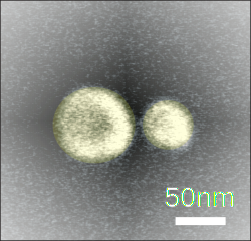
\includegraphics[width=15mm]{\currfiledir svg/particle_pair_SEM.png}};

\node at (600, 1.5) {single particle};	
\node at (690, 4) [left] {hybridized particle};	
	
    \end{axis}
    

    
\end{tikzpicture}

%\end{document}